Events with one prompt lepton produced in asociation with hadronic jets can pass the event selection if a jet is misidentified as a charged lepton or if a non-prompt lepton from the decay of a heavy flavor particle (such as $b$- and $c$-hadrons) passes the signal lepton criteria.
These misidentified jets and non-prompt leptons are collectively referred to as \emph{fake leptons}, or simply \emph{fakes}.
The rate at which a fake lepton is misidentified is generally not modelled well enough by the MC to accurately estimate their contributions directly from simulation.
Therefore, a data-driven technique called the \emph{fake factor} is used to estimate the size and shape of background processes from fake leptons.
In this analysis, a new modification to the fake factor is used involving the particle isolation variables; the method is outlined in the context of the \emph{default} fake factor in Section~\ref{ssww13tev:ff_method_default}, and the modified fake factor is outlined in Section~\ref{ssww13tev:ff_method_ptcone}.

%---------------------------------------------------------------------------------------------
%
%---------------------------------------------------------------------------------------------
\subsubsection{Overview of the default fake factor method}\label{ssww13tev:ff_method_default}
The goal of the fake factor method is to measure the fake rate in a region enriched in fake leptons and use it to estimate the size of the fake lepton background in a chosen signal or control region.
This is done by creating two samples of leptons: 
\begin{enumerate}
\item The \emph{nominal} sample is made up of leptons passing the signal selection.
\item The \emph{loose} sample is made up of leptons that fail the signal selection while still passing a loosened set of criteria.  This sample is enriched in fake leptons and is orthogonal to the set of signal leptons.
\end{enumerate}
Using the sets of nominal and loose leptons, a fake factor $f$ can be calculated in a region enriched in processes that are prone to producing fake leptons:
\begin{equation}
f = \frac{N_{\textrm{nominal}}}{N_{\textrm{loose}}}
\label{eq:ssww13tev_ff_default_unbinned}
\end{equation}
Since the fake rate is not expected to be constant over the entire phase space, the fake factor can be divided into bins in a chosen quantity:
\begin{equation}
f(b) = \frac{N_{\textrm{nominal}}(b)}{N_{\textrm{loose}}(b)}
\label{eq:ssww13tev_ff_default_binned}
\end{equation}
where $b$ represents the bin number.

In order to estimate the fake background contribution in a given signal or control region, the fake factor is applied to a second control region with a selection identical to the region of interest with one of the leptons required to satisfy the loose criteria.
The region for which the background is estimated contains two nominal leptons and is referred to as \emph{nominal+nominal} ($NN$), and the associated control region where the fake factor is applied contains one nominal and one loose lepton and is referred to as \emph{nominal+loose} ($NL$).
The fake background in a NN region can then be calculated as:
\begin{equation}
N_{NN}^{\textrm{fake\ bkg.}} = \sum\limits_{b}f(b) N_{NL}(b)
\label{eq:ssww13tev_ff_bkg_nosub}
\end{equation}

Backgrounds containing two prompt leptons can also enter the $NL$ region if one of the leptons passes the nominal selection and the other passes the loose selection.
Since the fake factor method estimates the fake background by scaling the amount of non-prompt events in the $NL$ region, if these prompt contributions are not be removed, they will be included in the scaling and the background will be overpredicted.
The final estimate of the fake background becomes:
\begin{equation}
N_{NN}^{\textrm{fake\ bkg.}} = \sum\limits_{b}f(b) \big(N_{NL}(b) - N_{NL}^{\textrm{prompt}}(b)\big)
\label{eq:ssww13tev_ff_bkg}
\end{equation}

%---------------------------------------------------------------------------------------------
%
%---------------------------------------------------------------------------------------------
\subsubsection{The fake factor with $\ptcone$}\label{ssww13tev:ff_method_ptcone}
When a jet produces a non-prompt lepton, that lepton only carries a fraction of the underlying jet's total momentum.
Due to the isolation cut applied to the nominal leptons, they typically carry a much larger percentage of the underlying jet momentum\footnote{Since the isolation variables are a measure of detector activity around the lepton, if other nearby particles carried a significant portion of the jet's momentum, the lepton would likely fail this cut.} than the loose leptons (which are allowed to fail this criteria).

This discrepancy in the underlying jet momentum fraction can cause problems in the calculation of the fake factor $f$.
Consider the case where two separate events have jets of identical momentum, but one produces a non-prompt lepton that passes the nominal selection, and the other produces a non-prompt lepton that passes the loose selection.
The loose lepton on average will have lower $\pt$ than the nominal lepton despite both originating from jets with the same momentum.
This can be seen explicitly when comparing the $\pt$ of a muon to its associated jet:
\begin{equation}
\Delta\pt(\mu,j) = \frac{\pt(j)-\pt(\mu)}{\pt(j)+\pt(\mu)}
\label{eq:ssww13tev_ff_deltapt}
\end{equation}
Since muons are not included in the jet reconstruction algorithm, $\Delta\pt$ approximates the momentum of the muon compared to the rest of the jet.
For muons that carry more than 50\% of the jet's momentum, $\Delta\pt$ will be negative and vice-versa.
The $\Delta\pt$ distributions for nominal and loose muons in $t\bar{t}$ MC events is shown Figure~\ref{fig:ssww13tev_ff_deltapt}, where a $50\gev$ jet on average corresponds to a $35\gev$ nominal muon and a $20\gev$ loose muon\footnote{To better illustrate the point, here the muon is added back into the jet $\pt$, and the corresponding muon $\pt$ is obtained via $\Delta\pt(\mu,j) = \frac{\big(\pt(j)-\pt{\mu}\big)-\pt(\mu)}{\big(\pt(j)-\pt(\mu)\big)+\pt(\mu)} = \frac{\pt(j)-2\pt(\mu)}{\pt(j)}$.}.

\begin{figure}[htbp]
  \centering
  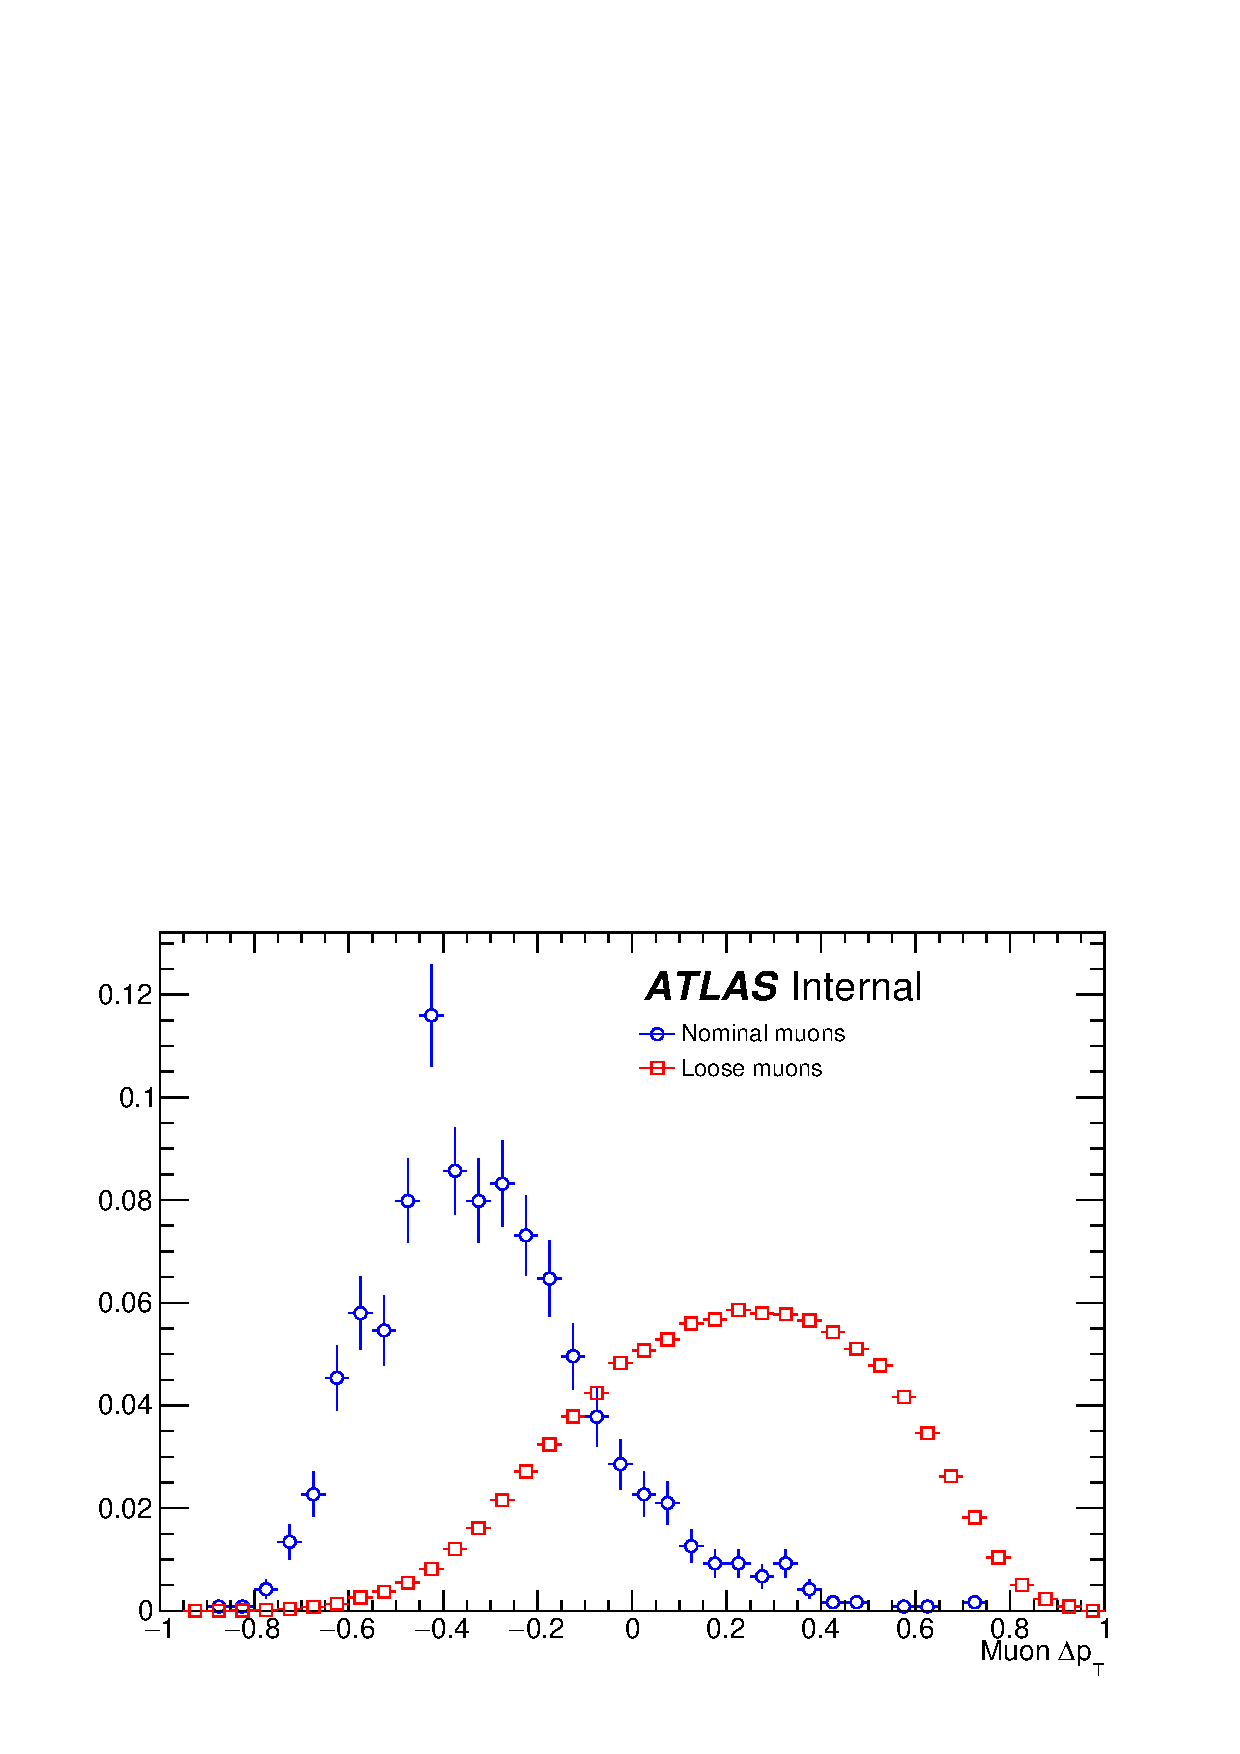
\includegraphics[width=.6\textwidth]{figs/ssww_13tev/backgrounds/ff/deltapt_ttbar}
  \caption{$\Delta\pt$ distributions for nominal (blue) and loose (red) muons in simulated $t\bar{t}$ events.  Each muon has been matched to a truth-level jet within a cone of $\deltar < 0.4$.  Both distributions are normalized to unit area.}
  \label{fig:ssww13tev_ff_deltapt}
\end{figure}

Since the default fake factor defined in Equation~\ref{eq:ssww13tev_ff_default_binned} is typically binned in lepton $\pt$, within a given bin, the underlying jet $\pt$ spectrum can differ substantially between the numerator and the denominator.
Additionally, these differences can vary depending on the process producing the non-prompt leptons or on the specific kinematic selections of the signal or control regions where the fake factor is applied.

Fortunately, the majority of the jet momentum not carried by the non-prompt lepton (excluding neutrinos) can be recovered using isolation variables.
A track-based isolation is chosen, referred to as $\ptcone$, and it contains the sum of the $\pt$ of all particle tracks originating from the primary vertex within a cone of $\deltar < 0.3$ around the lepton.
\TODO{Start here tomorrow -- finish up adding the $\ptptcone$ denominator explanation, add the dpt plots and one showing that $\ptcone$ is negligible for numerator etc}
Thus, the denominator of the fake factor is binned in $\ptptcone$ is chosen to represent the loose lepton

\begin{equation}
%f_b = \frac{N_{\textrm{nominal}}^b(\pt)}{N_{\textrm{loose}}^b(\ptptcone)}
f_b = \frac{N_{\textrm{nominal}}^{b(\pt)}}{N_{\textrm{loose}}^{b(\ptptcone)}}
\label{eq:ssww13tev_ff_ptcone_binned}
\end{equation}

%---------------------------------------------------------------------------------------------
%
%---------------------------------------------------------------------------------------------
\subsubsection{Implementation of the fake factor}\label{ssww13tev:ff_implementation}
The fake factor itself is measured from a sample of dijet events containing exactly one lepton and one $b$-jet that is approximately back-to-back with the lepton.
This $b$-jet requirement serves to enhance non-prompt lepton contributions while suppressing contributions from processes involving $W$ and $Z$ bosons.

\begin{figure}[htbp]
  \centering
  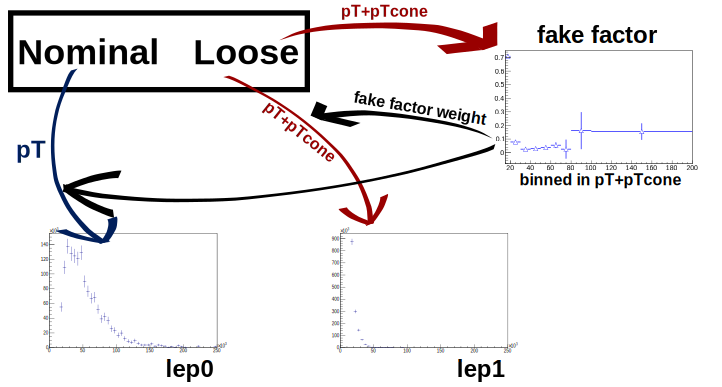
\includegraphics[width=.95\textwidth]{figs/ssww_13tev/backgrounds/ff/apply_ff}
  \caption{Graphical representation of the fake factor application using $\ptptcone$.  The value of $\ptptcone$ for the loose lepton is used to ``look up'' the fake factor weight which is then applied to the event.  The loose lepton's $\pt$ becomes $\ptptcone$ for the purpose of the fake background estimation.}
  \label{fig:ssww13tev_ff_application}
\end{figure}

%---------------------------------------------------------------------------------------------
%
%---------------------------------------------------------------------------------------------
\subsubsection{Results of the fake factor}\label{ssww13tev:ff_results}

\begin{figure}[htbp]
  \centering
  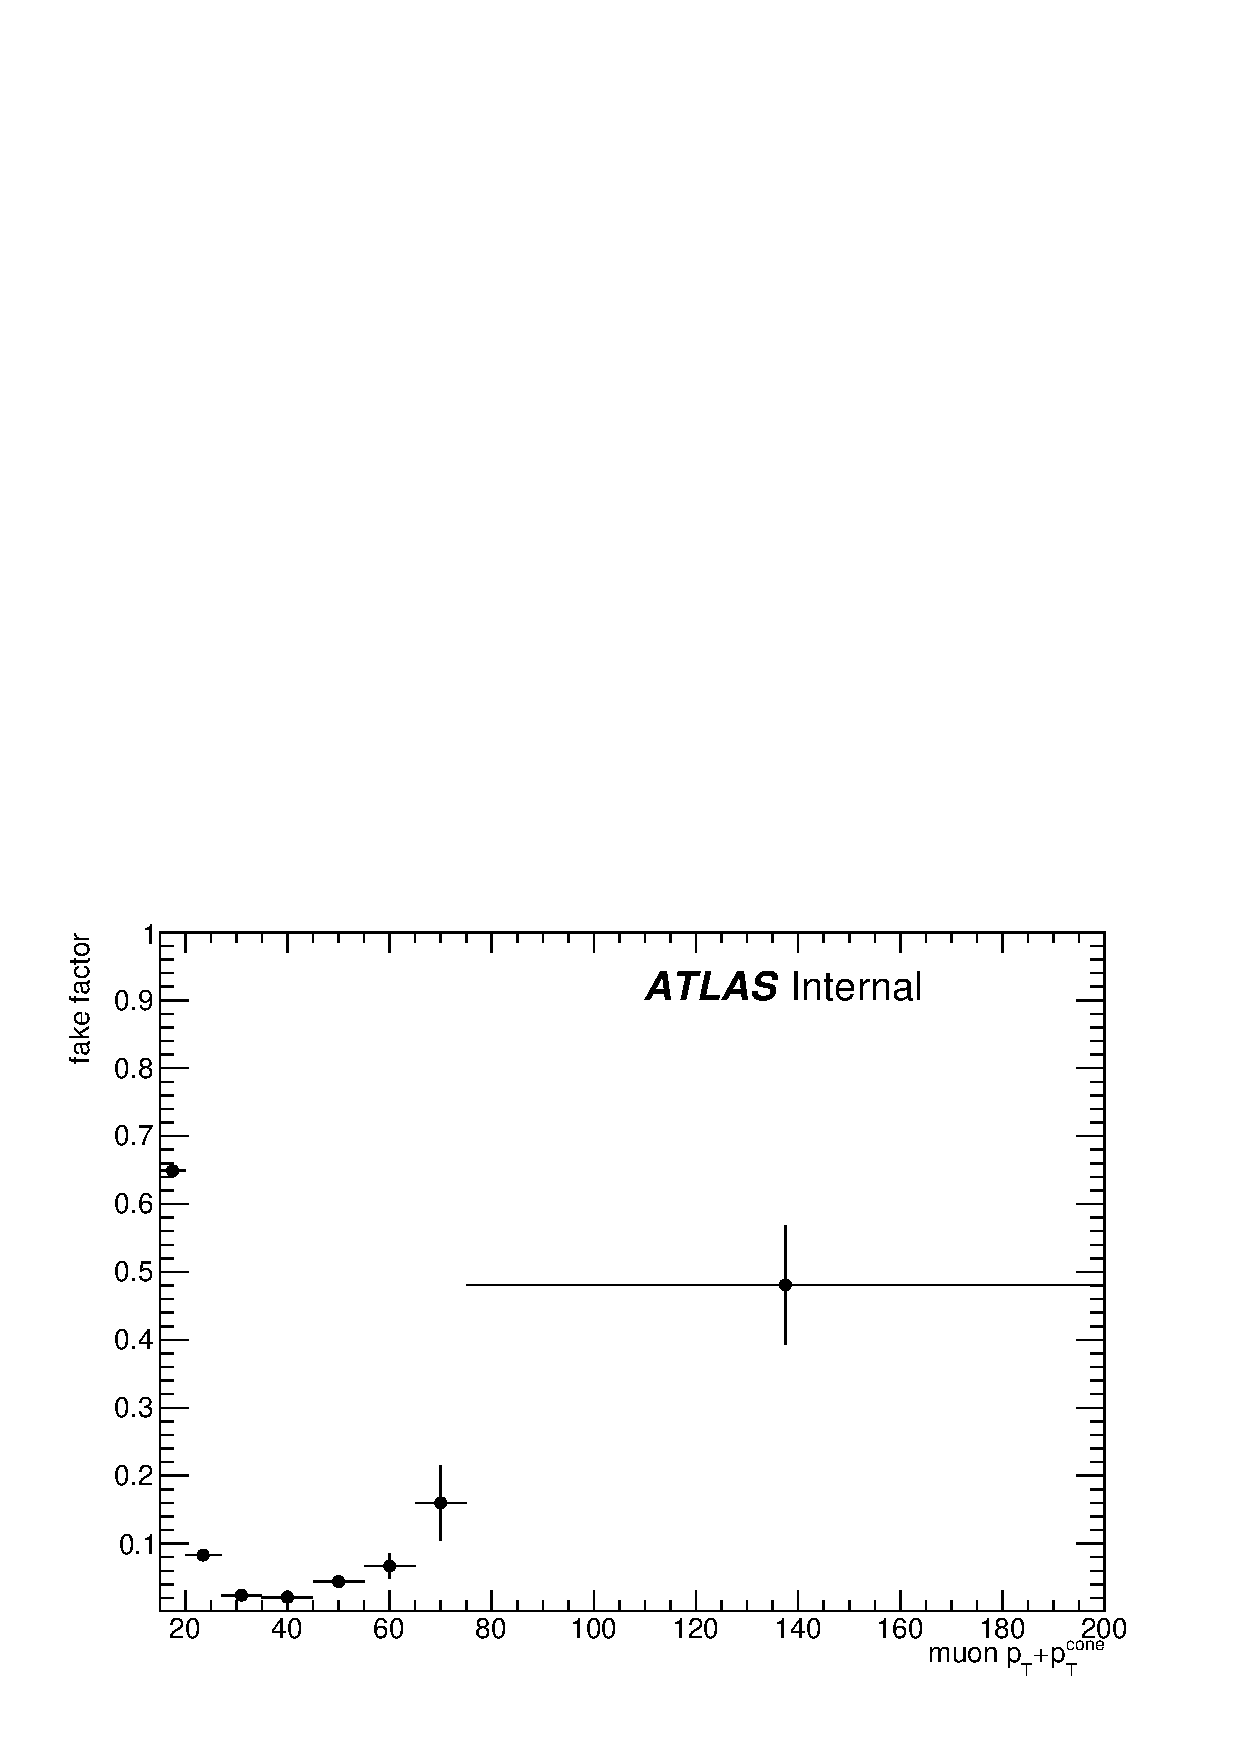
\includegraphics[width=.6\textwidth]{figs/ssww_13tev/backgrounds/ff/muon_ff}
  \caption{The measured fake factor as a function of muon $\ptptcone$.  The error bars represent the statistical uncertainty only.}
  \label{fig:ssww13tev_ff_muon}
\end{figure}

\begin{figure}[htbp]
  \centering
  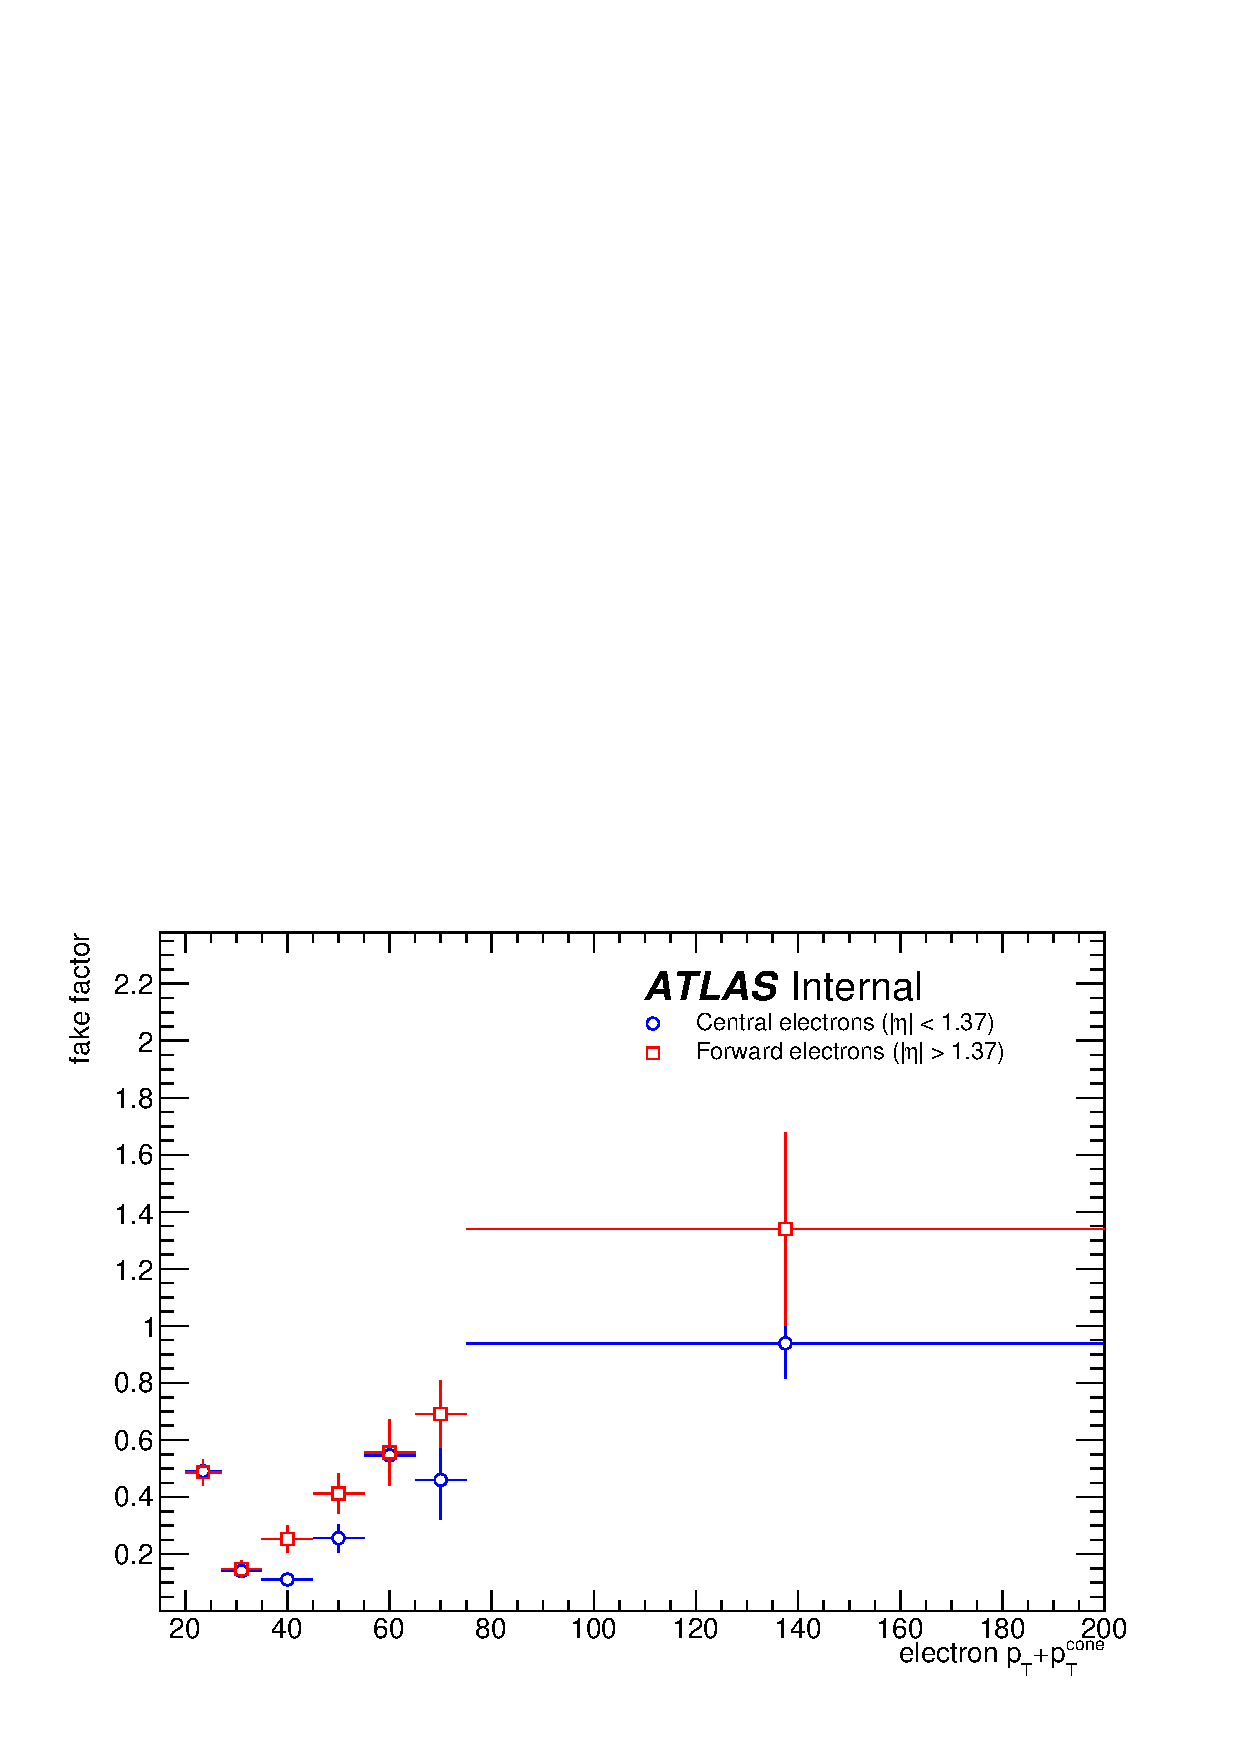
\includegraphics[width=.6\textwidth]{figs/ssww_13tev/backgrounds/ff/elec_ff}
  \caption{The measured fake factor as a function of electron $\ptptcone$ in the central ($|\eta|<1.37$, blue) and forward ($|\eta| > 1.37$, red) regions of the detector.  The error bars represent the statistical uncertainty only.}
  \label{fig:ssww13tev_ff_elec}
\end{figure}

\subsubsection{Test of fake factor in validation regions}\label{ssww13tev:ff_vr}

\subsubsection{Systematic uncertainties}\label{ssww13tev:ff_systematics}

\begin{figure}[htbp]
  \centering
  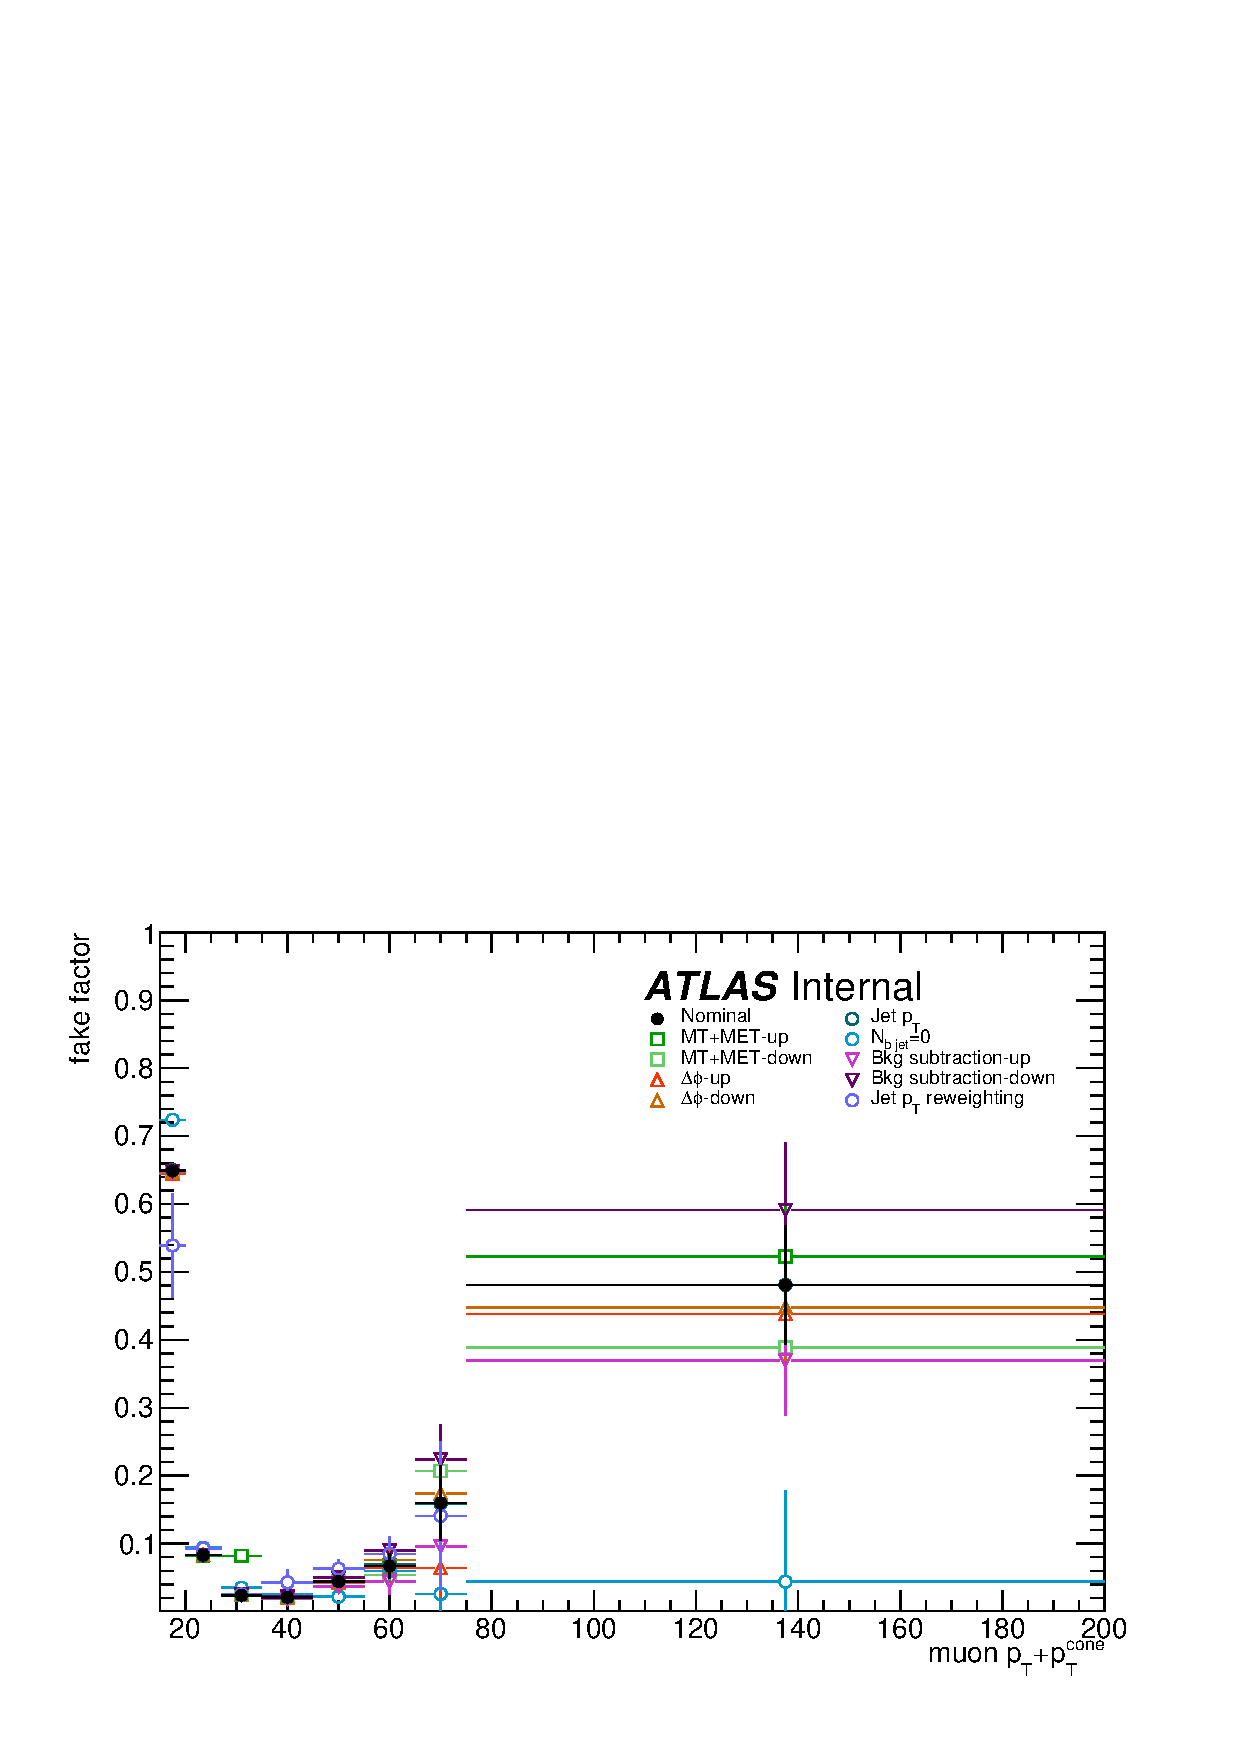
\includegraphics[width=.6\textwidth]{figs/ssww_13tev/backgrounds/ff/muon_ff_sys}
  \caption{Systematic variations in the fake factor as a function of muon $\ptptcone$.  The individual fake factors obtained for each systematic variation are displayed with their statistical uncertainties.}
  \label{fig:ssww13tev_ff_muon_sys}
\end{figure}

\begin{figure}[htbp]
  \centering
  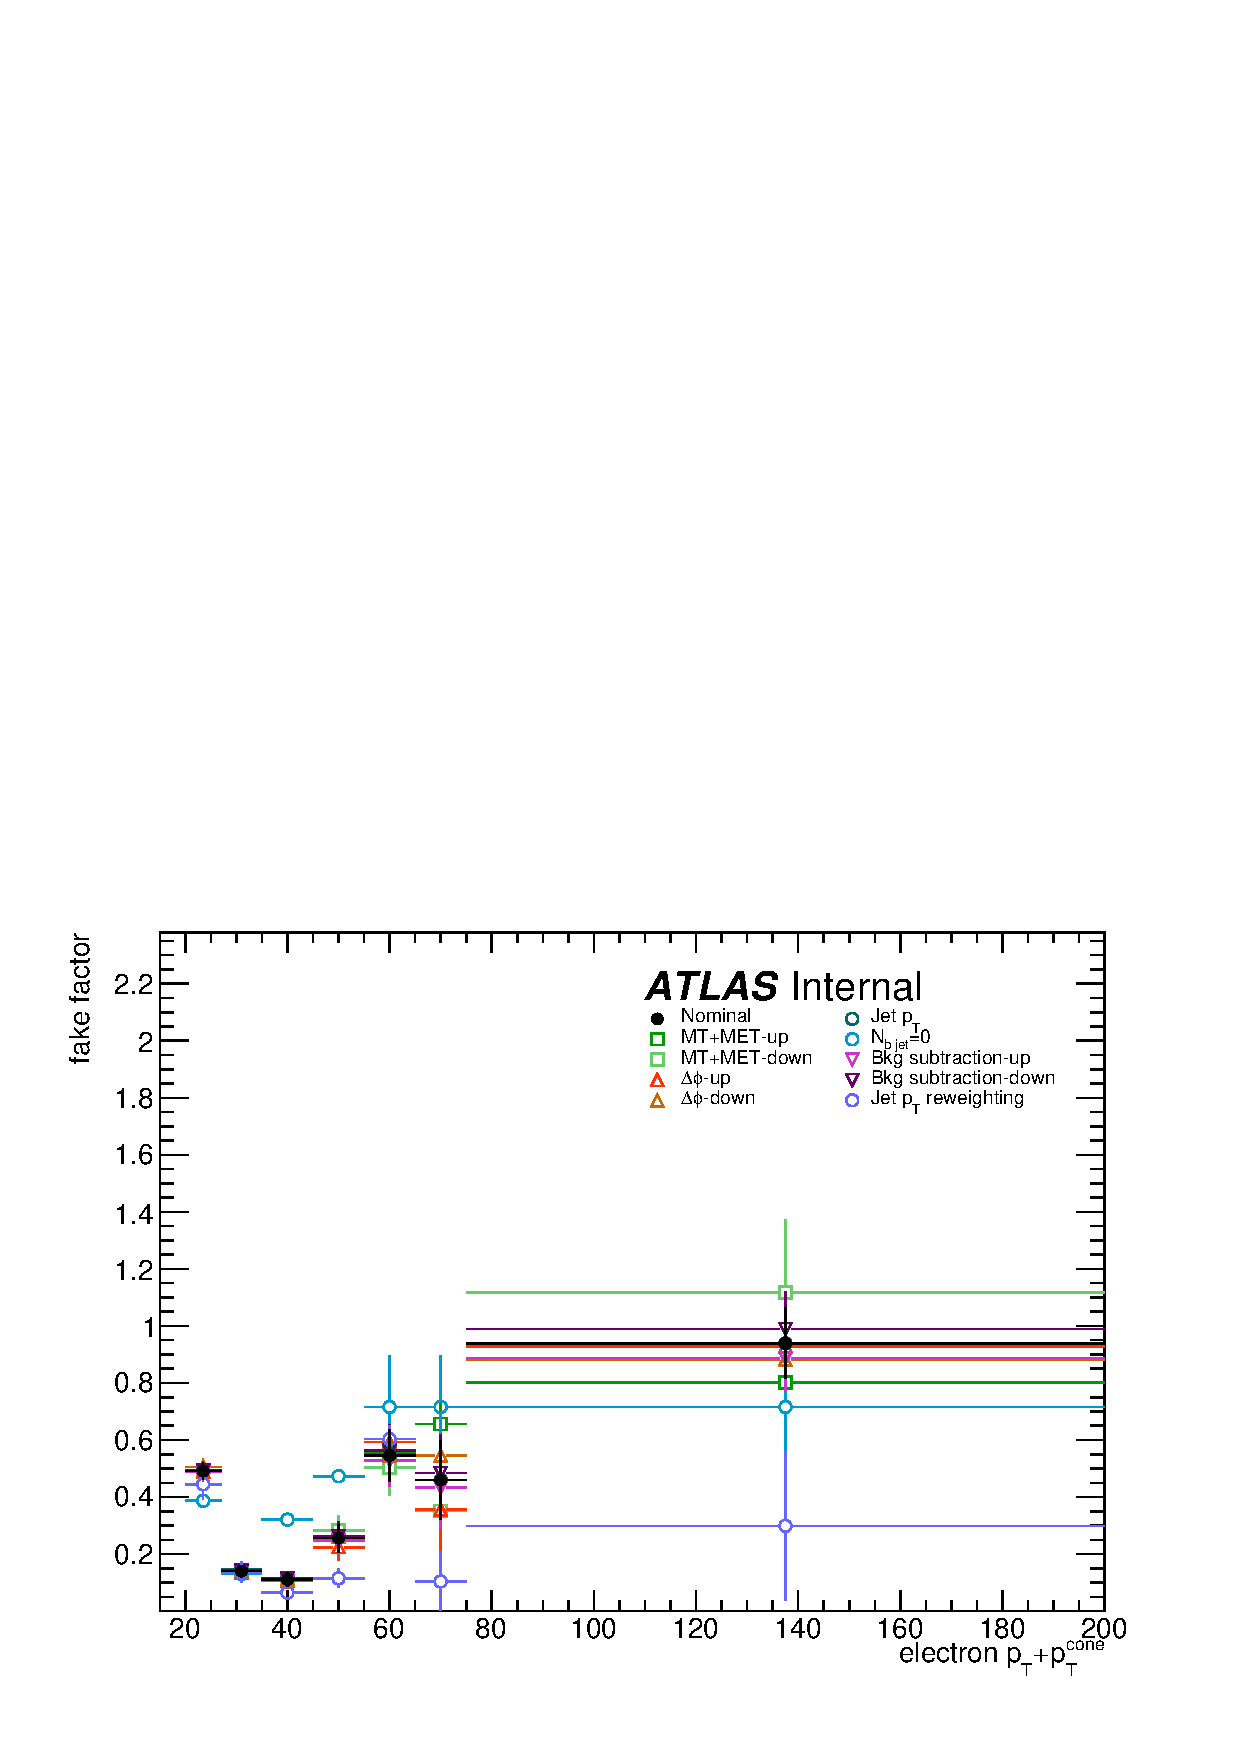
\includegraphics[width=.6\textwidth]{figs/ssww_13tev/backgrounds/ff/elec_central_ff_sys}\\
  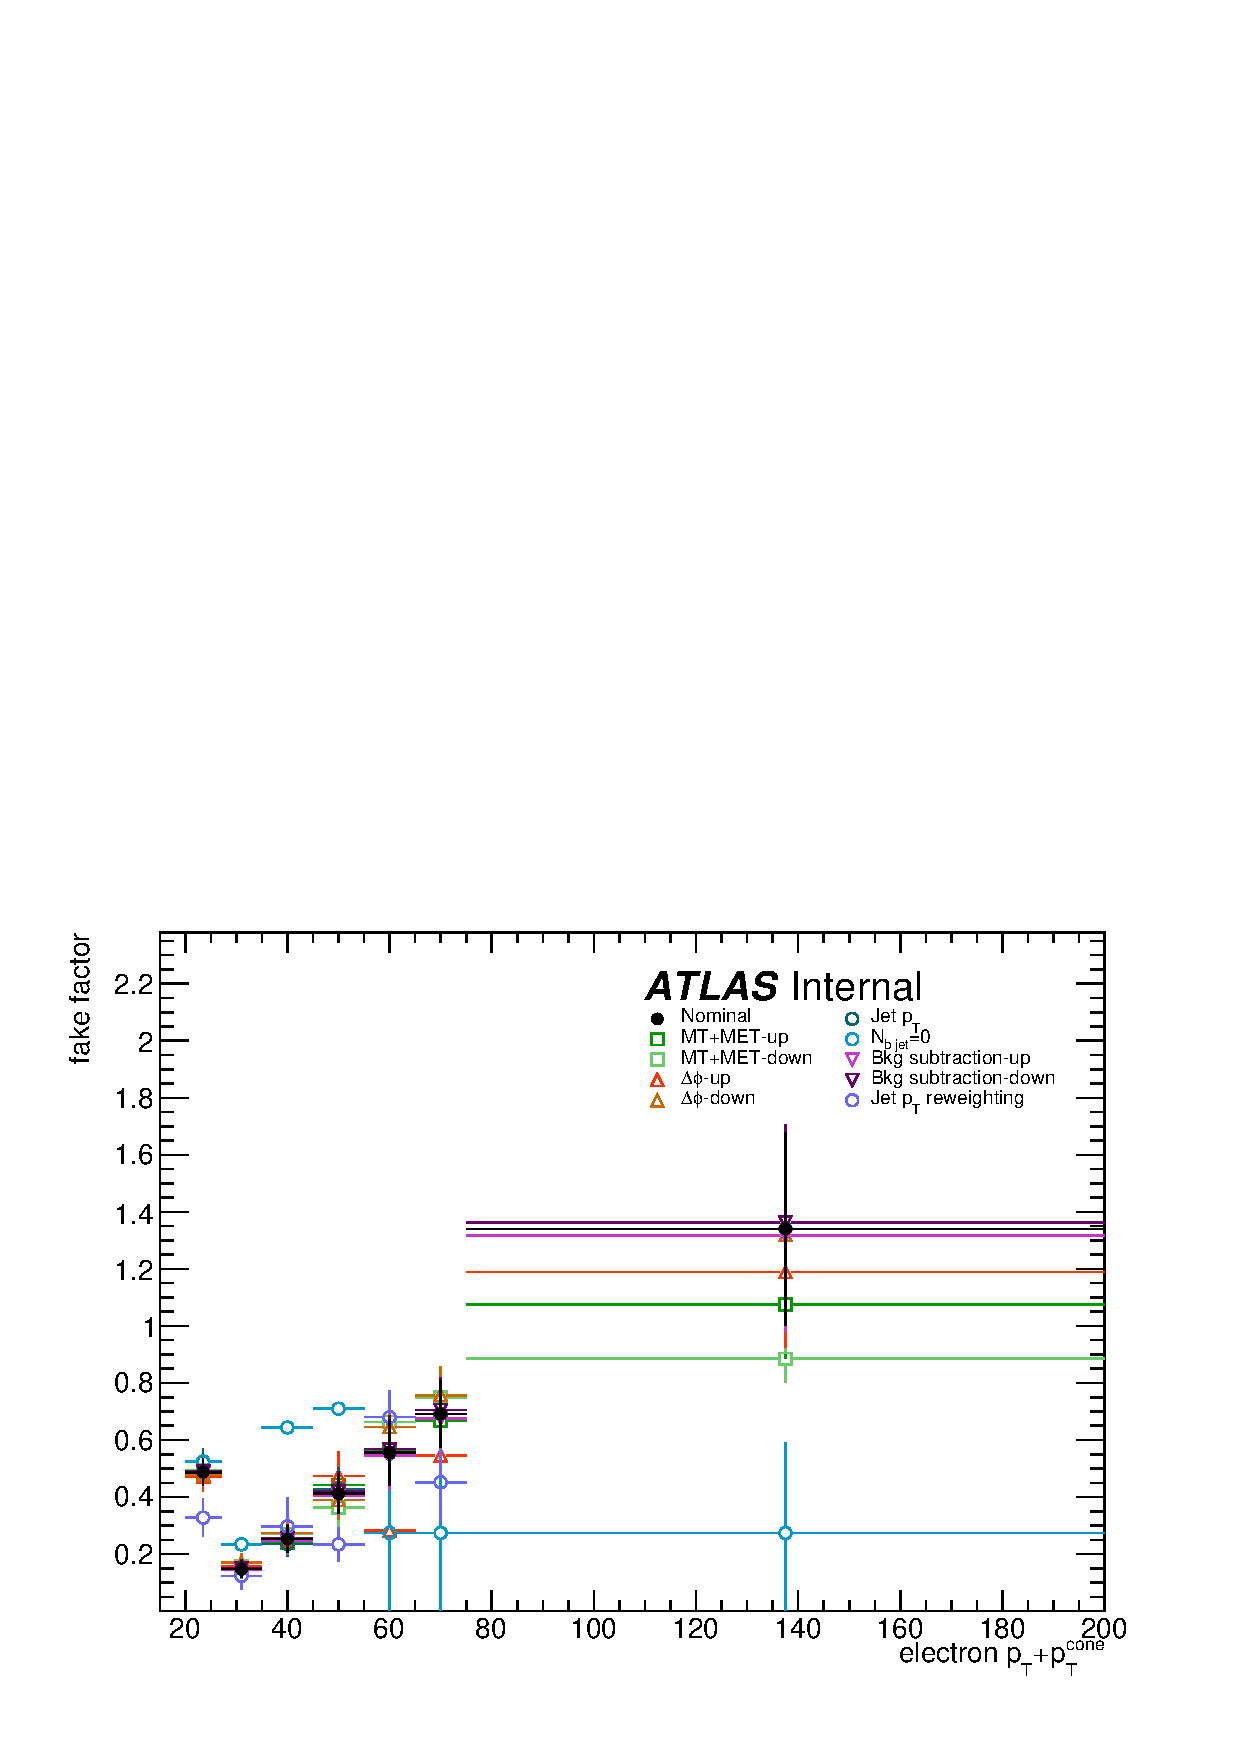
\includegraphics[width=.6\textwidth]{figs/ssww_13tev/backgrounds/ff/elec_forward_ff_sys}
  \caption{Systematic variations in the fake factor as a function of electron $\ptptcone$ in the central ($|\eta|<1.37$, top) and forward ($|\eta| > 1.37$, bottom) regions of the detector.  The individual fake factors obtained for each systematic variation are displayed with their statistical uncertainties.}
  \label{fig:ssww13tev_ff_elec_sys}
\end{figure}
